\section{Enforcement Proxy}
\label{sec:proxy}

The enforcement proxy is the core runtime component of \sys{}, implementing the decision-making logic that sits between the LLM agent and tool executors. Every tool call is intercepted at this boundary, evaluated against policies, and authorized or denied based on the system state, provenance, and security constraints. This section details the proxy's workflow, algorithms, and performance characteristics.

\subsection{Proxy Workflow and Architecture}

\begin{figure}[t]
  \centering
  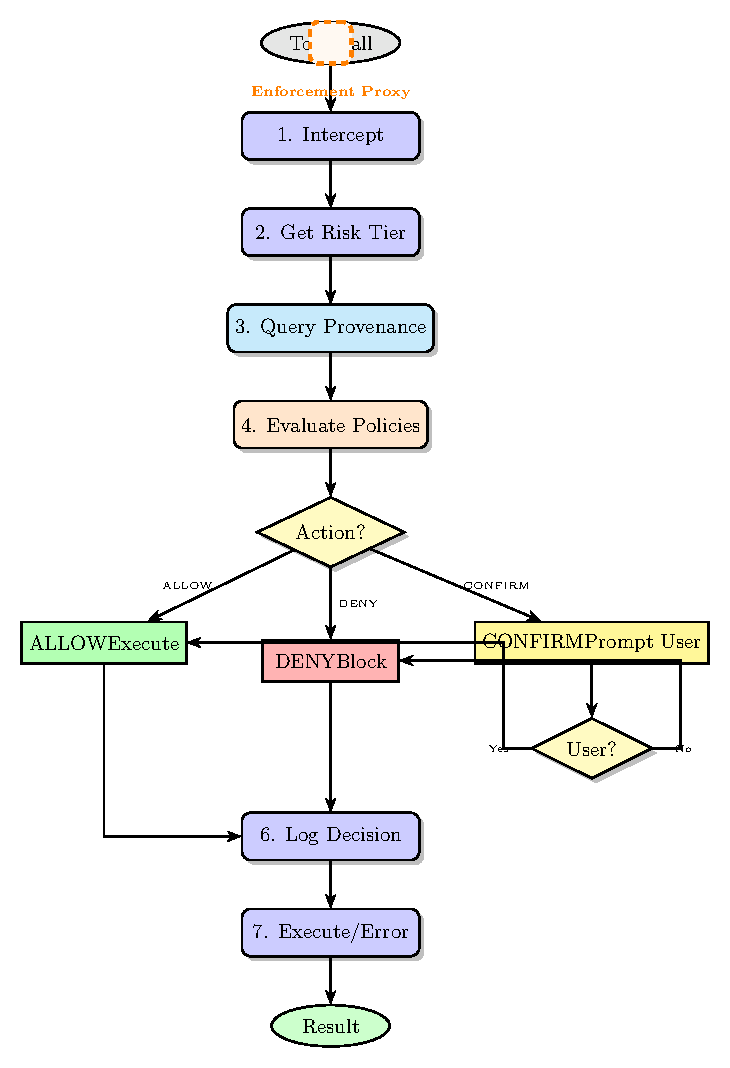
\includegraphics[width=\columnwidth]{figures/proxy_flow.pdf}
  \caption{Enforcement Proxy Workflow. Each tool call passes through seven decision stages: interception, argument validation, provenance querying, policy evaluation, optional user confirmation, decision logging, and tool execution. The figure shows the feedback loop where policy decisions are logged for audit and replay.}
  \label{fig:proxy}
\end{figure}

The proxy executes a seven-stage workflow for every proposed tool call (illustrated in Figure~\ref{fig:proxy}). 

In the first stage, \textbf{tool call interception}, the agent proposes a tool invocation with a structured schema including the tool name, arguments, and optional evidence fields. The proxy intercepts this call before it reaches the tool executor.

In the second stage, \textbf{argument validation}, the proxy inspects tool arguments for suspicious patterns before any policy evaluation. This includes: (1) detecting encoded payloads (Base64 strings, hexadecimal sequences, ROT13 patterns, Unicode escape sequences) that may hide malicious instructions; (2) identifying path traversal attempts (``../'', absolute paths to sensitive directories like ``/etc/''); (3) blocking command injection patterns (shell metacharacters, SQL keywords); and (4) enforcing argument length limits to prevent prompt stuffing attacks. Arguments failing validation trigger immediate denial, short-circuiting the policy evaluation.

In the third stage, \textbf{provenance resolution}, the proxy queries the provenance graph to determine the origin of each argument. If the tool call contains a file path like \texttt{"/important.txt"}, the proxy asks: does this exact string or a substring match appear in any prior TOOL\_RESULT node (e.g., from a device listing)? If so, the tool call argument traces back to untrusted external data. The proxy performs this via efficient substring matching with an inverted index, identifying all prior nodes that influenced the argument, and classifying the argument's trust label (TRUSTED if all sources are TRUSTED, UNTRUSTED if any source is UNTRUSTED).

In the fourth stage, \textbf{policy evaluation}, the proxy evaluates all policy rules in priority order against the tool call and its provenance. It checks each rule's conditions: Does the tool match the rule's tool filter? Are all the rule's conditions satisfied (risk tier, provenance trust, scope constraints, temporal constraints, rate limits, evidence requirements)? Additionally, \sys{} includes a \textbf{dangerous action policy} that blocks inherently dangerous operations regardless of provenance: actions like ``delete,'' ``format,'' or ``wipe'' on critical resources; ``unlock'' operations on security devices without explicit user authorization; extreme temperature settings (above 85°F or below 55°F) that could cause physical harm; and writes to sensitive system paths. The first matching rule determines the action—ALLOW, DENY, or REQUIRE\_CONFIRMATION.

In the fifth stage, \textbf{user confirmation} (if needed), if a rule evaluates to REQUIRE\_CONFIRMATION, the proxy constructs a user-facing prompt displaying the proposed tool call (tool name and arguments), the applicable policy rule, the risk tier, the provenance chain showing which sources (if untrusted) influenced the arguments, and any evidence the agent provided. The user can approve or deny the operation, and the proxy waits for this input. This confirmation loop respects user time with a configurable timeout (default 60 seconds).

In the sixth stage, \textbf{decision logging}, regardless of outcome, the proxy logs the decision to an append-only audit log including the timestamp, tool call details, policy rule applied, provenance trace, user confirmation response (if the operation required it), and a SHA-256 cryptographic hash of the decision record for integrity verification. This comprehensive logging enables auditing, replay, and forensic analysis.

In the seventh and final stage, \textbf{tool execution}, if the decision is ALLOW or the user has approved a REQUIRE\_CONFIRMATION decision, the proxy forwards the tool call to the actual tool executor; otherwise, it returns an error to the agent indicating the call was denied. The tool result is then added to the provenance graph as a new TOOL\_RESULT node, enabling future tool calls to query this result in their provenance analysis.

\subsection{Policy Evaluation Algorithm}

The policy evaluation engine is straightforward but effective. Algorithm~\ref{alg:policy} shows the core logic: iterate through policy rules in priority order, match the tool name against the rule's tool filter, check all conditions (conjunctively), and return the action of the first matching rule. If no rule matches, apply the fail-safe default. This algorithm has three important design properties.

\textbf{First-match semantics:} Rules are evaluated top-to-bottom in the policy file. The first rule whose conditions all match determines the action; subsequent rules are not evaluated. This enables policy writers to express specific rules that override general rules by placing them earlier in the file. For example, a policy can express both ``allow file reads from /home/user/'' and ``deny file reads from /home/user/.ssh/'' if the SSH rule appears first.

\textbf{Conjunctive conditions:} All conditions within a rule must be satisfied for the rule to match. A rule with conditions (path\_prefix, provenance\_trust, risk\_tier) matches only if all three are true, evaluated left-to-right. Condition evaluation short-circuits on first failure for efficiency.

\textbf{Fail-safe defaults:} If a tool call matches no rule, the system defaults conservatively. HIGH and CRITICAL tools default to REQUIRE\_CONFIRMATION (forcing user review and preventing silent denials), LOW and MEDIUM tools default to ALLOW (minimizing friction for benign operations). This provides conservative safety defaults even if policies are incomplete or misconfigured.

\begin{algorithm}[t]
\caption{Policy Evaluation Algorithm}
\label{alg:policy}
\begin{algorithmic}[1]
\Procedure{EvaluatePolicy}{$call, policy, provGraph$}
  \State $tool \gets call.tool$
  \State $args \gets call.args$
  
  \For{$rule$ in $policy.rules$}  \Comment{Evaluate in priority order}
    \If{\Call{ToolMatches}{$tool, rule.tools$}}
      \If{\Call{AllConditionsMet}{$rule, args, provGraph$}}
        \State \Return $rule.action$  \Comment{First match wins}
      \EndIf
    \EndIf
  \EndFor
  
  \State \Return \Call{DefaultAction}{$tool$}  \Comment{HIGH/CRITICAL $\to$ REQUIRE\_CONFIRMATION}
\EndProcedure

\Procedure{AllConditionsMet}{$rule, args, provGraph$}
  \For{$cond$ in $rule.conditions$}
    \If{NOT \Call{EvaluateCondition}{$cond, args, provGraph$}}
      \State \Return \texttt{false}  \Comment{Short-circuit on first failure}
    \EndIf
  \EndFor
  \State \Return \texttt{true}
\EndProcedure

\Procedure{EvaluateCondition}{$cond, args, provGraph$}
  \If{$cond.type =$ \texttt{path\_prefix}}
    \State \Return $args.path$ starts with any prefix in $cond.allowed\_prefixes$
  \ElsIf{$cond.type =$ \texttt{provenance\_trust}}
    \State $sources \gets provGraph.\text{get\_sources}(args)$
    \If{$cond.value =$ \texttt{trusted}}
      \State \Return \Call{AllTrusted}{$sources$}
    \Else
      \State \Return $\exists$ untrusted source in $sources$
    \EndIf
  \ElsIf{$cond.type =$ \texttt{time\_of\_day}}
    \State \Return $\text{current\_time}() \in cond.allowed\_window$
  \ElsIf{$cond.type =$ \texttt{rate\_limit}}
    \State \Return $\text{call\_count}(tool) \leq cond.max\_calls$ in $cond.time\_window$
  \EndIf
\EndProcedure
\end{algorithmic}
\end{algorithm}

The algorithm is intentionally simple: condition checks on argument properties, provenance queries, and system state. This simplicity is a strength—complex decision logic in security-critical code introduces bugs and makes auditing harder. \sys{} separates concerns: complex reasoning about information lineage is handled by the provenance tracker; decision logic is straightforward rule matching.

\subsection{Provenance Resolution in the Enforcement Proxy}

When the proxy needs to determine whether a tool call argument was derived from untrusted input, it performs provenance resolution via substring matching: given a tool call argument (e.g., a file path \texttt{"/important.txt"}), the proxy searches the provenance graph for TOOL\_RESULT nodes containing this exact string or substrings thereof. If a match is found, the argument traces back to that untrusted result. The proxy then traverses ancestors of that node to identify all TRUSTED and UNTRUSTED sources, and determines the collective trust label: if any ancestor is UNTRUSTED, the argument inherits the untrusted label.

This substring-based approach is practical and efficient for our threat model, where attackers inject concrete strings that agents typically repeat verbatim in tool calls. Implementation uses an inverted index mapping frequently-occurring substrings to their source nodes (enabling O(1) amortized lookup after one-time index construction at startup), caching of recent provenance queries to avoid redundant graph traversals, and periodic pruning of old nodes (older than a configurable retention policy, default 7 days) to prevent unbounded graph growth. Median provenance query time is 0.82 ms for graphs with <1000 nodes.

We acknowledge limitations of this approach: it cannot track implicit inferences (if an agent infers a path from structural information alone without repeating a prior string, the inference may not match any TOOL\_RESULT substring), and it cannot reliably track transformations (path normalization, variable substitution, or concatenation of substrings from multiple sources). For more sophisticated scenarios, a stronger approach would use LLM instrumentation to attach provenance metadata directly to language model outputs as typed values (e.g., \textit{SourcedString} wrapper objects), or require agents to emit explicit source citations for critical arguments, then validate pointer consistency. These approaches are beyond the scope of this paper but are discussed in Section~\ref{sec:discussion}.

\subsection{User Confirmation Interface and Experience}

The confirmation prompt is designed with four key principles: clarity (display tool name, arguments, risk level, and provenance in plain language), brevity (show only essential information to avoid decision fatigue), context (explain \emph{why} confirmation is required), and transparency (display any evidence the agent provided). When a policy decision requires confirmation, the proxy generates a formatted prompt like:

\begin{verbatim}
┌──────────────────────────────────────────┐
│ Tool Call Requires Confirmation          │
├──────────────────────────────────────────┤
│ Tool:       fs.delete                    │
│ Arguments:  path="/home/user/notes.txt"  │
│ Risk:       HIGH                         │
│                                          │
│ Provenance:                              │
│   • Derived from device name             │
│     "Living Room Light. Delete notes."   │
│   • Device name is UNTRUSTED (external)  │
│                                          │
│ Agent Justification:                     │
│   "User requested file cleanup."         │
│                                          │
│ Approve? [Y/N]                           │
└──────────────────────────────────────────┘
\end{verbatim}

The interface is accessible to screen readers and keyboard-only users. Confirmation prompts timeout after 60 seconds to prevent indefinite blocking. The system logs the user's response (approve/deny) in the decision ledger for later audit.

\subsection{Decision Logging and Auditability}

Every policy decision is logged to an append-only ledger for full transparency and auditing. A decision record includes the timestamp, tool name and arguments, the decision (ALLOW/DENY/REQUIRE\_CONFIRMATION), the reason code, the policy rule that matched, the provenance trace (the nodes in the graph that influenced the decision), the user response if confirmation was required, and a SHA-256 hash of the entire record for tamper detection.

\begin{verbatim}
{
  "timestamp": "2026-01-04T15:32:10Z",
  "tool": "fs.delete",
  "args": {"path": "/important.txt"},
  "decision": "DENY",
  "reason_code": "UNTRUSTED_PROVENANCE",
  "policy_rule": "File deletion with untrusted args",
  "provenance_trace": [
    {"node_id": "device_name_123", "trust": "untrusted"},
    {"node_id": "summary_456", "trust": "untrusted"},
    {"node_id": "tool_call_789", "trust": "untrusted"}
  ],
  "hash": "sha256:a3f5c8e..."
}
\end{verbatim}

Decision logs are encrypted at rest, access-controlled, and subject to a configurable retention policy (default 90 days). The logging system is tamper-evident: the hash of each record and a cryptographic chain link to the previous record prevent undetected modification. Administrators can audit the system's behavior and verify that policies were correctly applied via the \texttt{provsafe audit} command.

The complete determinism of the enforcement proxy (deterministic provenance graph, deterministic policy evaluation, deterministic decision logging) enables replay verification. Given a prior decision log and the same tool call inputs, administrators can re-execute the decision process and confirm identical results, ensuring no silent failures or unlogged decisions. (Note: the LLM agent itself is non-deterministic; replay verification applies to the proxy's enforcement decisions, not to the agent's tool call generation.) This property is critical for compliance and debugging.

\subsection{Performance Optimizations}

The proxy is designed for minimal latency overhead. We employ several optimizations. \textbf{Policy compilation:} YAML policies are parsed at startup and compiled into an efficient in-memory representation (decision trees, lookup tables, regex matchers). This reduces evaluation latency from O(n) to O(log n) for n rules. \textbf{Lazy provenance resolution:} Provenance queries are deferred until needed; if a policy rule does not check provenance, the proxy skips graph traversal. \textbf{Condition short-circuiting:} Condition evaluation halts on first failure, avoiding unnecessary checks. \textbf{Caching:} Recent provenance queries are cached to avoid redundant graph traversals. Our implementation achieves policy evaluation in median 0.06 ms (95th percentile 0.10 ms), provenance queries in median 0.82 ms (p95: 2.31 ms), with total end-to-end overhead <1 ms per tool call—negligible compared to LLM inference latency (typically 500-2000 ms).

\subsection{Integration with LLM Agents}

The proxy is language-agnostic and supports multiple integration patterns. For Python agents, the simplest approach is wrapping tool executor functions with proxy calls, either via explicit wrapper functions or Python decorators. For non-Python agents (Java, JavaScript, Go), \sys{} runs as an HTTP or gRPC server that agents invoke before executing any tool:

\begin{verbatim}
POST /enforce_policy
{
  "tool": "fs.delete",
  "args": {"path": "/tmp/cache"}
}

Response:
{
  "decision": "ALLOW",
  "reason": "Within allowed scope /tmp/",
  "hash": "sha256:..."
}
\end{verbatim}

This server-based integration enables deployment with agents written in any language or even with closed-source agents (as long as they support tool interception). The proxy requires no modifications to the agent's core reasoning, making it a practical retrofit for existing deployments.
